The version 1 website colour scheme is an amalgamation of white (for the background) and orange (for miscellaneous design features). The white background leverages on its simplicity and clarity, an important criteria for retaining the attention of the user. Moreover, the orange colour is reportedly stimulating for the users appetite. \footnote{[ http://desktoppub.about.com/cs/colorselection/p/orange.htm ]}. The group also agreed on an orange logo design. 

\subsection{Version 1}

\begin{figure}
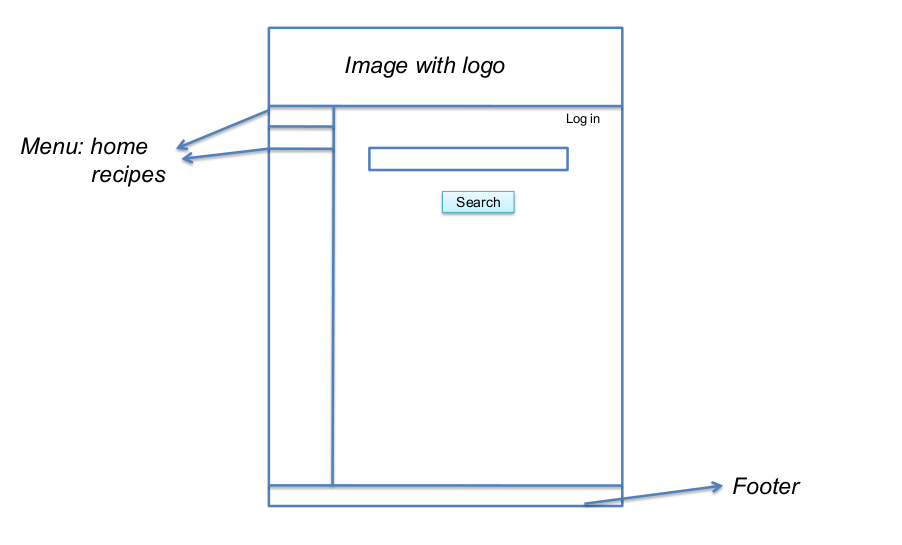
\includegraphics[width=0.9\textwidth]{home_page}
\caption{Layout of the Home Page}
\label{fig:home_page}
\end{figure}

The merit of the version 1 website design is in its simplicity. Upon accessing the website, (Fig~\ref{fig:home_page}) users are presented there are three drop-down menus which allows people to select ingredients. The drop-down menus are transversely positioned to accommodate the vertical cascading of the ingredients of the menus. Users are provided with three menus to select ingredients and submit a search. This then links to the recipe list page. Additionally, the “recipes” button in the sidebar links the page to the complete list of recipes alphabetically.

\begin{figure}
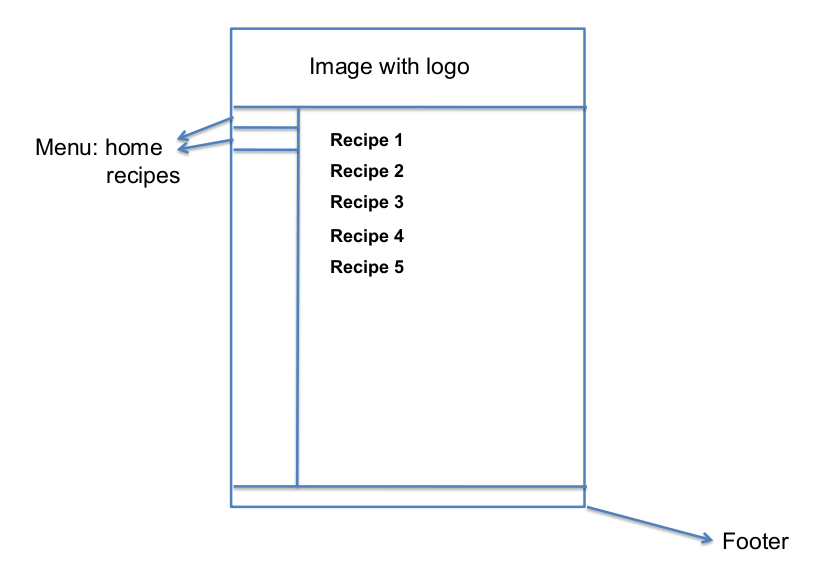
\includegraphics[width=0.9\textwidth]{recipe_list_page}
\caption{Layout of the Recipe List Page}
\label{fig:recipe_list}
\end{figure}

The recipe list page (Fig~\ref{fig:recipe_list}) contains a list of recipes with at least one of the three ingredients. However, the recipe may contain other ingredients which were not specified by the user. Upon recipe selection, the specific recipe page will be displayed.

\begin{figure}
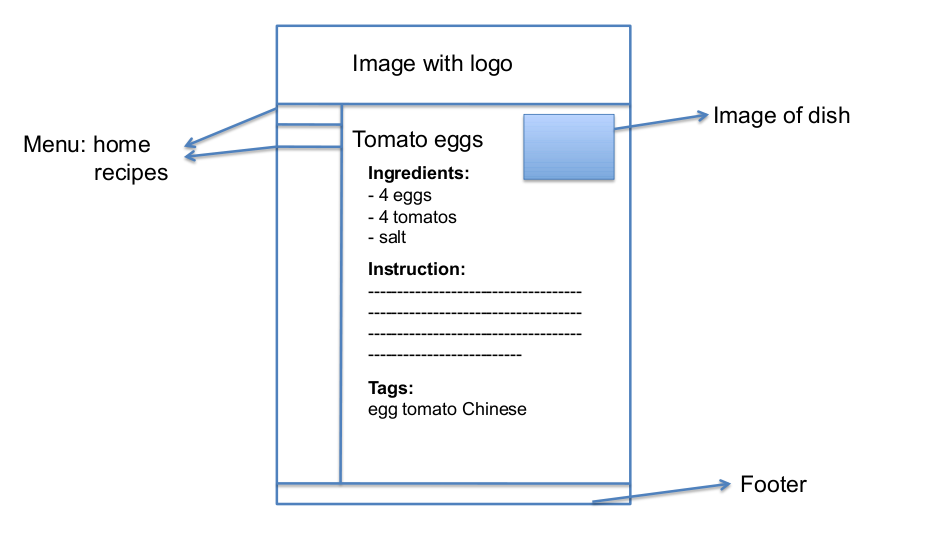
\includegraphics[width=0.9\textwidth]{recipe_page}
\caption{Layout of the Recipe Page}
\label{fig:recipe_page}
\end{figure}

The recipe page (Fig \ref{fig:recipe_page}) contains recipe details, for example recipe name, ingredients, the instruction, and recipe tags.
 
One design limitation of version 1 is that the website only has three drop-down menus, and the user is unable to type in ingredients. Being a prototype, the version 1 database is fitted with few recipes hence such functionality is redundant. 

\subsection{Version 2}
Version 2 is an upgraded version of the original version containing more functions (described by the Product Specification). With the use of technology such as JAVA Script, the web interface will look more polished. Users will be able to enter text data into ingredient selection text boxes, which will have the tab completion feature for ingredients instead of using a drop-down menu. There will also be a larger database of ingredients hence justifying the use of tab completion as apposed to drop-down menus.

Additionally, for version 2, users are allowed to have web accounts. With this account, a user can have their own history of recipes ratings. There will also be links on the website linking to the most popular recipes. And once the user has logged in, the home page will also have an area that gives suggest recipes based on past rating. 

For the recipe page, with the image of the recipe, a new area called “You might like” would be also added.  This area is also made up of a list of brief look of recipes. These recipes are chosen from the database using collaborative filtering techniques. In addition, users, at this point, could click the tags and get a list of recipes that contains this tag.
The last but not the least, we will also have a simple web view for mobile phone and other portable equipment (iTouch, psp, etc). This mobile view is only simple black and white appearance with the same function as the version 1, which could be accessed through the internet.

\subsection{Version 3}
The ideal version, which is the third version of digichef, would not only have a more friendly website based on version 2 but also a mobile application that user could actually install. And the recipes are searchable by more than ingredients, for instance, the region of this recipe (Chinese dish) or other category like vegetarian. 
With the increasing of the whole database and tag system, the home page would also have the area contains the most popular tags. When the user click on a typical tag, the website would update with a list of recipes which ordered by rates. 
Once the user want to rate recipe, the webpage would open a feedback dialog box which allows user to rate it vary from one star to five stars, and also allows user to leave their own command about this recipes. And a number of the latest command would be showed on the exact recipe page. 
A huge improvement of version 3 is that user could upload their own recipes. When they construct the new recipe, they need to provide the name, the ingredients, the instruction and also the tag to classify the recipe. Thus, the new version of recipe page would be same as version 2 but with author’s name. 

